\section{Directional Completion Tracks Object Geometry}
\label{sec:reflection}

The complete Phase-A screen in Fig.~\ref{fig:screening} contains five DROID/RoboLab and three RoboTwin rows. Large RIGHT-over-LEFT marginal gaps appear for $\pi_{0.5}$ and DreamZero. GR00T is floor-limited at $3/27$ LEFT versus $0/27$ RIGHT and is the only row whose small observed difference favors LEFT; Nano is near ceiling, and the RoboTwin gaps are small. Later experiments use registered checkpoint subsets, with geometric claims further restricted by endpoint-redirection controls. The screen is neither an architecture ranking nor a pooled cross-arena estimate.

\subsection{Position reflection}

We hold the robot, cameras, fixed geometry, prompts, checkpoints, and seeds constant while reflecting the centers of movable objects about the sagittal plane. Each of three DROID/RoboLab checkpoints uses 27 seeds and four cells (two directions by two layouts), for 108 episodes. The $\pi_{0.5}$ reflection cohort uses seeds 9400--9426, independently of the Phase-A screen at 8303--8329. Thus Fig.~\ref{fig:screening} reports $5/27$ LEFT and $24/27$ RIGHT, whereas the control cell below contains $4/27$ and $25/27$. The primary outcome is the within-seed layout interaction in requested-side depth; success is secondary because binary outcomes can saturate by layout and direction.

\begin{figure*}[t]
  \centering
  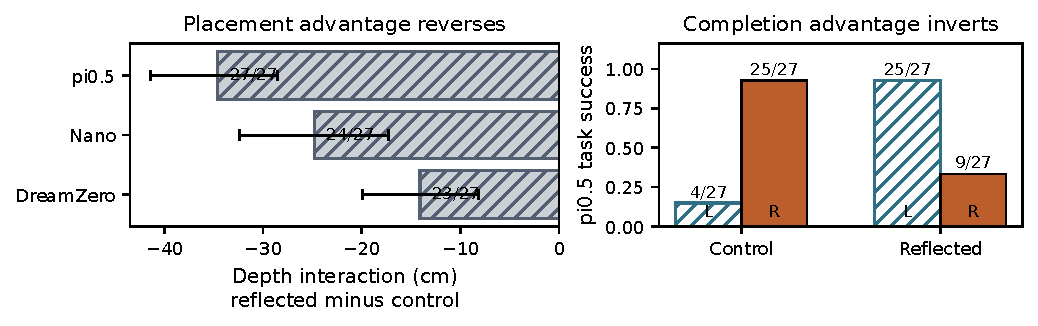
\includegraphics[width=0.98\textwidth]{figures/reflection_core.pdf}
  \caption{\textbf{Reflecting movable-object positions reverses placement advantage.}
  Left: reflected-minus-control interaction in requested-side depth, with seed-clustered 95\% bootstrap intervals; fractions give seeds with the negative interaction. Right: $\pi_{0.5}$ task completion in the independent reflection cohort. Nano is near a binary ceiling, while DreamZero changes from low control completion to near-ceiling reflected completion; their continuous depth interactions remain the common estimand.}
  \label{fig:reflection}
\end{figure*}

As Fig.~\ref{fig:reflection} shows, requested-side depth reverses in every checkpoint: $-34.6$\,cm for $\pi_{0.5}$ (95\% CI $[-41.4,-28.5]$; $27/27$ seeds; $p=1.49\times10^{-8}$), $-24.8$\,cm for Nano ($[-32.4,-17.3]$; $24/27$; $p=4.92\times10^{-5}$), and $-14.1$\,cm for DreamZero ($[-19.9,-8.2]$; $23/27$; $p=3.11\times10^{-4}$). For Nano and $\pi_{0.5}$, the estimated interactions in canonical endpoint redirection are much smaller, $+0.5$\,cm and $-1.12$\,cm (both $p=.701$). Because equivalence was not established for those estimates, we do not call redirection invariant; the supported contrast is that placement changes far more than the estimated redirection interaction.

For $\pi_{0.5}$, binary completion itself inverts. The control layout yields $4/27$ LEFT versus $25/27$ RIGHT successes; reflection yields $25/27$ versus $9/27$, a difference-in-differences of $-1.37$ ($p=5.96\times10^{-8}$). The checkpoint, prompts, seeds, controller, and robot are unchanged. The benchmark's favored direction changes when the movable objects change sides.
